\documentclass{beamer}
%
% Choose how your presentation looks.
%
% For more themes, color themes and font themes, see:
% http://deic.uab.es/~iblanes/beamer_gallery/index_by_theme.html
%
\mode<presentation>
{
  \usetheme{default}      % or try Darmstadt, Madrid, Warsaw, ...
  \usecolortheme{default} % or try albatross, beaver, crane, ...
  \usefonttheme{default}  % or try serif, structurebold, ...
  \setbeamertemplate{navigation symbols}{}
  \setbeamertemplate{caption}[numbered]
} 

\addtobeamertemplate{navigation symbols}{}{%
    \usebeamerfont{footline}%
    \usebeamercolor[fg]{footline}%
    \hspace{1em}%
    \insertframenumber/\inserttotalframenumber
}

\usepackage[english]{babel}
\usepackage[utf8x]{inputenc}
\usepackage{xcolor}

\definecolor{myblue}{RGB}{68, 114, 196}
\definecolor{mygreen}{RGB}{0, 176, 80}

\title[Završni rad]{Klasifikacija uporabom umjetnih
neuronskih mreža}

\author{Darijo Brčina}
\institute{Sveučilište u Zagrebu \linebreak \textbf{Fakultet elektrotehnike i računarstva} \linebreak \linebreak Završni rad br. 6950}
\date{Zagreb, 06.07.2020}

\begin{document}

\begin{frame}
  \titlepage
\end{frame}

% Uncomment these lines for an automatically generated outline.
\begin{frame}{Sadržaj}
  \tableofcontents
\end{frame}

\section{Opis zadatka}
	\begin{frame}{Opis zadatka}
		Cilj:
		\begin{itemize}
			\item naučiti neuronsku mrežu da na temelju danih labeliranih podataka jasno može odrediti kojem razredu pripadaju
		\end{itemize}

		\bigskip
		\bigskip
		
		\begin{figure}
			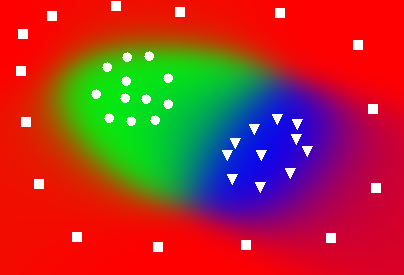
\includegraphics[scale=0.5]{img/cilj_slika.png}
		\end{figure}
	\end{frame}

\section{Nadzirano učenje}
	\begin{frame}{Nadzirano učenje}
		\begin{itemize}
			\item Jedno od glavnih područja strojnog učenja
			\item Model nadziranog učenja (engl. \textit{supervised learning}) prolazi kroz dvije faze:
			\bigskip
			\begin{figure}
			    \pause
			    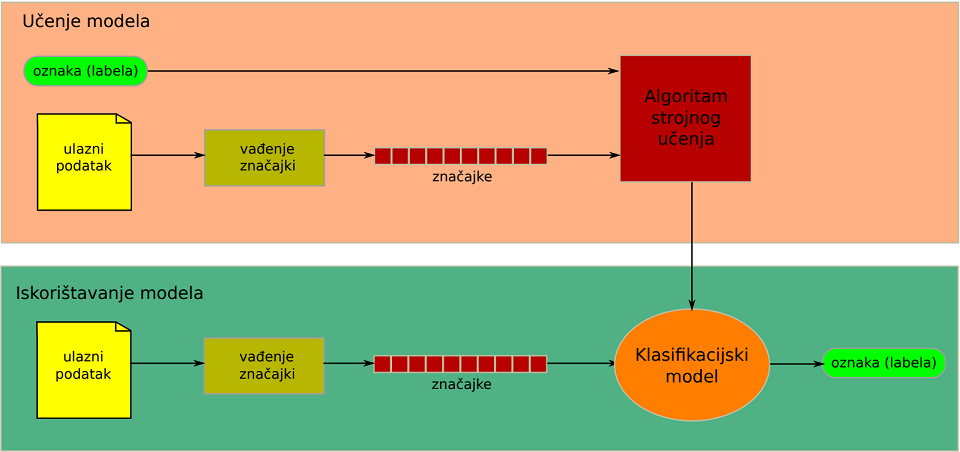
\includegraphics[scale=0.35]{img/supervised-learning-flow.png}
		    \end{figure}
		    \bigskip
		    \pause
		    \item Glavni cilj je omogućiti da model razvije svojstvo \textbf{generalizacije}
		    \item Ispostavlja se da je to dosta zahtjevno za izvesti pa često dolazi do problema \textbf{prenaučenosti} (engl. \textit{overfitting})
		\end{itemize}
	\end{frame}
	\begin{frame}{Lijek za prenaučenost}
	    \begin{itemize}
	        \item Prenaučenost je jedan od glavnih problema strojnog učenja koji model čini beskorisnim zbog loše generalizacije
	        \item Jedan od načina kako spriječiti prenaučenost je korištenje metode \textbf{unakrsna provjera} (engl. \textit{cross-validation})
	        \item Ideja je da se oko 30\% uzoraka \textbf{skupa za učenje} (engl. \textit{training set}) prebaci u \textbf{skup za provjeru} (engl. \textit{validation set}) te prati pogreška nad oba skupa pomoću koje ćemo odrediti kada je učenje modela potrebno zaustaviti:
	        \smallskip
	        \pause
	        \begin{figure}
			    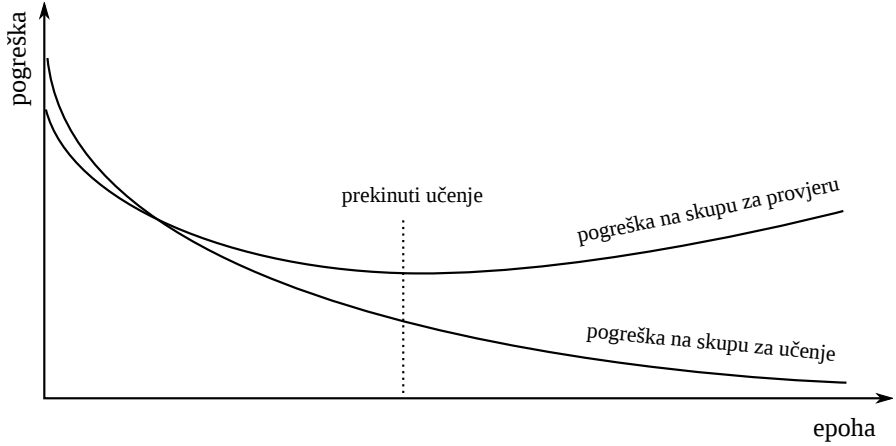
\includegraphics[scale=0.35]{img/cross-validation.png}
		    \end{figure}
	    \end{itemize}
	\end{frame}
    \begin{frame}{Skup za testiranje}
        \begin{itemize}
            \item Ponekad su modeli složeni pa je potrebno odrediti njihovu optimalnu složenost te se zbog toga uvodi \textbf{skup za testiranje} (engl. \textit{testing set}) koji također sadrži oko 30\% uzoraka skupa za učenje i služi za provjeru točnosti jednom naučenog modela
            \item Slikovito prikazani skupovi:
            \bigskip
            \begin{figure}
			    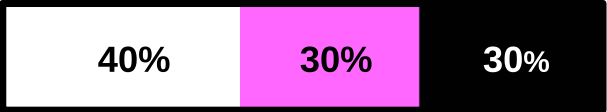
\includegraphics[scale=0.35]{img/skupovi.png}
		    \end{figure}
        \end{itemize}
    \end{frame}

\subsection{Problemi nadziranog učenja}
    \subsubsection{Regresija}
        \begin{frame}{Problemi nadziranog učenja - Regresija}
            \begin{itemize}
                \item Regresija (engl. \textit{regression}) je tehnika kojom se pokušava modelirati odnos između određenog broja značajki i kontinuirane ciljne varijable
                \item Razlikujemo više tipova regresija poput linearne i nelinearne 
                regresije kao i regresije s jednom varijablom i regresije s više varijabli
                \pause
                \begin{figure}
                    \begin{subfigure}
                        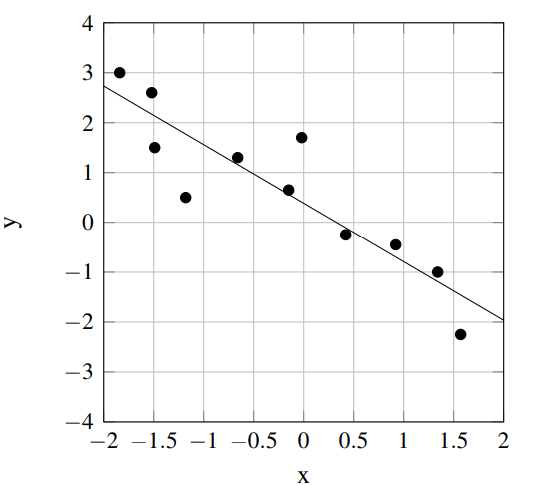
\includegraphics[scale=0.3]{img/linear-regression.png}
                    \end{subfigure}
                    \begin{subfigure}
                        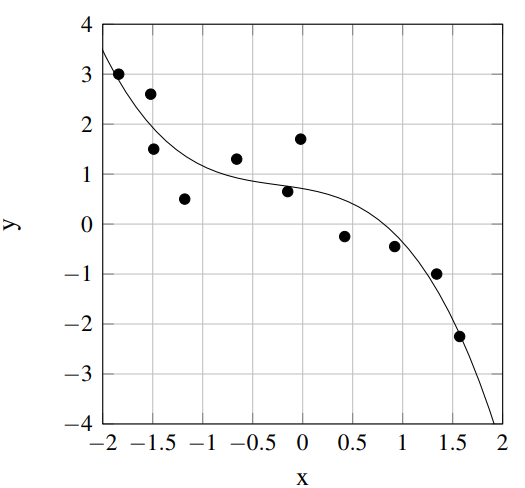
\includegraphics[scale=0.3]{img/polynom-regression.png}
                    \end{subfigure}
                \end{figure}
            \end{itemize}
        \end{frame}
    \subsubsection{Klasifikacija}
        \begin{frame}{Problemi nadziranog učenja - Klasifikacija}
            \begin{itemize}
                \item Klasifikacija (engl. \textit{classification}) je tehnika kojom se određene oznake pokušavaju kategorizirati diskretnim vrijednostima
                \item Kao i kod regresije, razlikujemo linearnu i nelinearnu klasifikaciju
                \item Razlikujemo binarnu i višerazrednu klasifikaciju i klasifikaciju više oznaka
                \bigskip
                \pause
                \begin{figure}
                    \begin{subfigure}
                        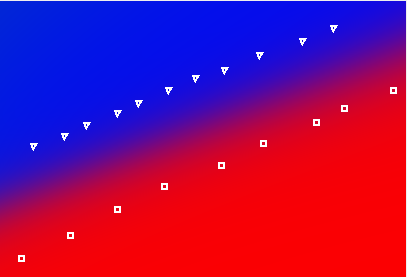
\includegraphics[scale=0.35]{img/linear-classification.png}
                    \end{subfigure}
                    \begin{subfigure}
                      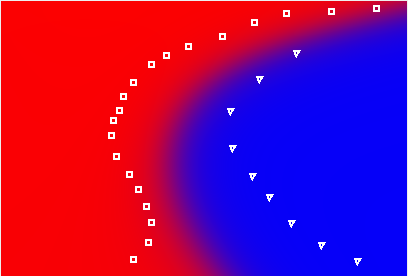
\includegraphics[scale=0.35]{img/non-linear-classification.png}
                    \end{subfigure}
                \end{figure}
            \end{itemize}
        \end{frame}

\section{Umjetne neuronske mreže}
    \begin{frame}{Umjetne neuronske mreže}
        \begin{itemize}
            \item Jedan od najkorištenijih algoritama strojnog učenja
            \item Motivacija pronađena u građi, povezanosti i brzini obrade raznih podražaja ljudskog mozga te mogućnosti učenja iz prijašnjeg iskustva
            \item Danas je poznato da u ljudskom mozgu postoji oko 10\textsuperscript{11} neurona te 10\textsuperscript{15} međusobnih veza, što znači da je svaki neuron u prosjeku povezan s 10\textsuperscript{4} različitih veza
            \item Primjer konektivističkog pristupa
            \item Područje koje se bavi proučavanjem umjetnih neuronskih mreža naziva se neuro računarstvo (engl. \textit{neuro-computing}) koje je jedno od grana mekog računarstva (engl. \textit{soft-computing}) 
        \end{itemize}
    \end{frame}
    \begin{frame}{Umjetne neuronske mreže}
        \begin{figure}
            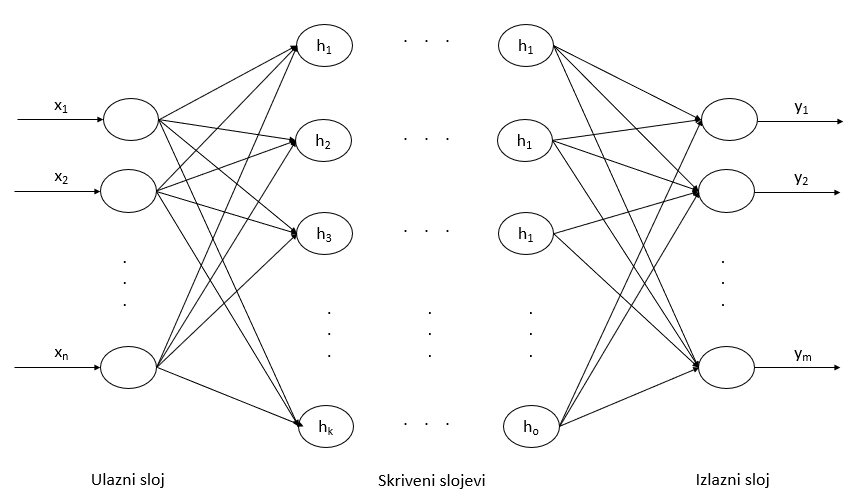
\includegraphics[scale=0.3]{img/ann.png}
        \end{figure}
        \begin{figure}
            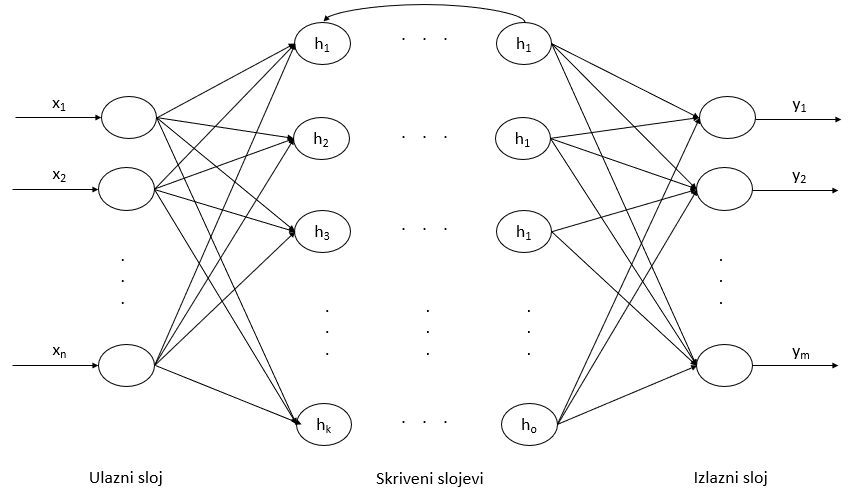
\includegraphics[scale=0.3]{img/cycle-ann.png}
        \end{figure}
    \end{frame}
    
    \subsection{Umjetni neuron}
        \begin{frame}{Umjetni neuron}
            \begin{itemize}
                \item Motiviran strukturom biološkog neurona:
                \begin{figure}
                    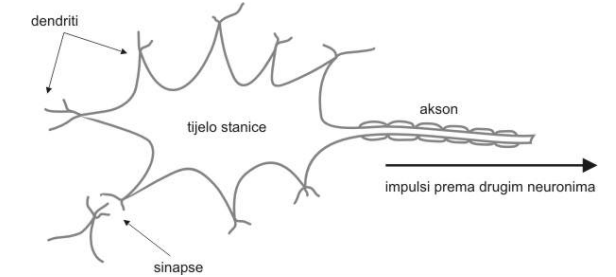
\includegraphics[scale=0.5]{img/bio-neuron.png}
                \end{figure}
                \item Definiran 1943.\ u radu \textit{A Logical Calculus of Ideas Immanent in Nervous Activity} dvojice znanstvenika Warren S. McCulloch i Walter H. Pitts
            \end{itemize}
        \end{frame}
        \begin{frame}{Umjetni neuron}
           \begin{itemize}
                \begin{figure}
                    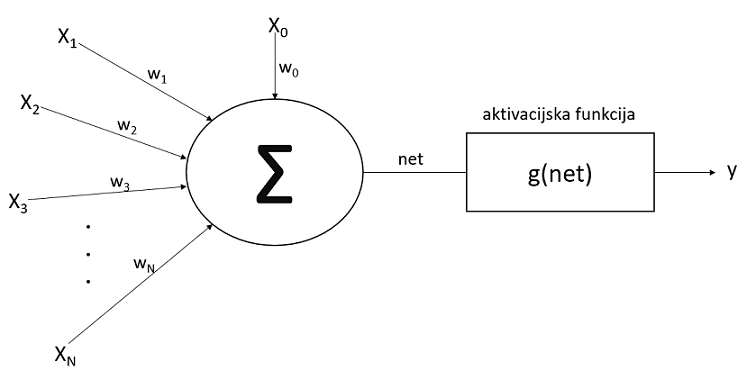
\includegraphics[scale=0.36]{img/ai-neuron.png}
                \end{figure}
                \item Sastoji se od $(n+1)$ različitih ulaza \textbf{x} i težina \textbf{w} te jednog izlaza \textbf{y}
                \item Izlaz se dobije tako što se prvo izračuna \textbf{net} vrijednost po formuli: \[net = \sum\limit_{i=0}^Nx\textsubscript{i} \cdot w\textsubscript{i}\]
                \item Zatim se dobivena \textbf{net} vrijednost provuče kroz neku od aktivacijskih funkcija
            \end{itemize}
        \end{frame}
        
    \subsection{Aktivacijske funkcije}
        \begin{frame}{Aktivacijske funkcije}
            \begin{itemize}
                \item U starijoj literaturi nazivane i prijenosnim funkcijama
                \item Nalaze se tik prije izlaza neurona i određuju hoće li neuron biti aktiviran ili ne, tj.\ hoće li se "paliti" ili ne
                \item Razlikujemo binarnu funkciju skoka (engl. \textit{step function}), linearne aktivacijske funkcije poput funkcije identiteta (engl. \textit{identity function}) i nelinearne aktivacijske funkcije poput sigmoidalne (engl. \textit{sigmoid function}), funkcije zglobnice (engl. \textit{Rectified Linear Unit, ReLU}) i dr.
                \item Svaka od njih različito utječe na izgled \textbf{decizijskih granica}, granica između razreda nastalih rezultatom klasifikacije
                \item Danas se najviše koriste nelinearne aktivacijske funkcije zbog toga što su derivabilne i čije derivacije nisu konstante što uvelike pospješuje učenje mreža
                \item Funkcija skoka se koristi kod binarne klasifikacije, linearne funkcije kod linearno interpretabilnih problema, a nelinearne se mogu koristiti gotovo uvijek
            \end{itemize}
        \end{frame}
        \begin{frame}{Aktivacijske funkcije}
            \begin{figure}
                \begin{subfigure}
                    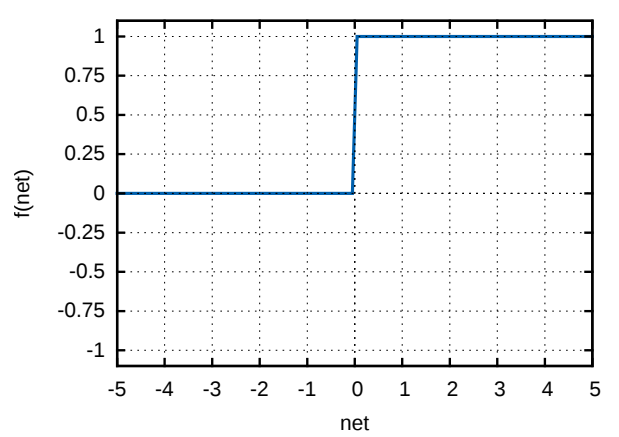
\includegraphics[scale=0.23]{img/step-fun.png}
                \end{subfigure}
                \begin{subfigure}
                    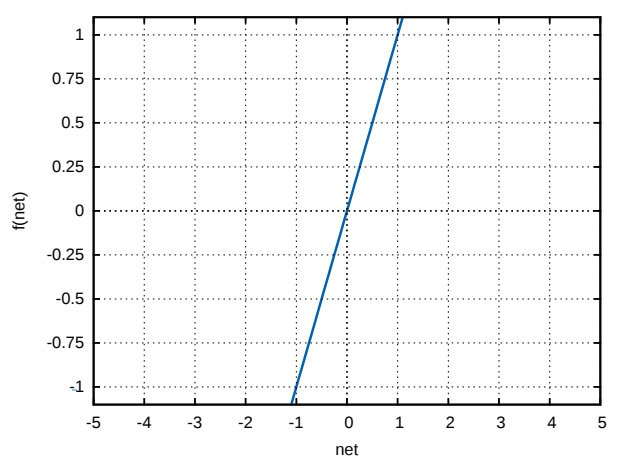
\includegraphics[scale=0.22]{img/id-fun.png}
                \end{subfigure}
                \begin{subfigure}
                    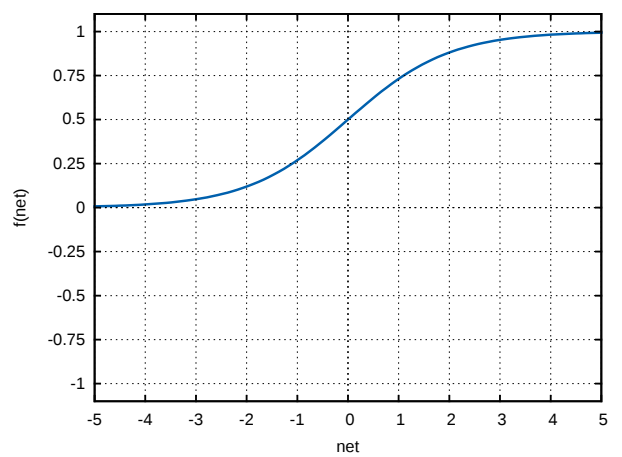
\includegraphics[scale=0.22]{img/sigm-fun.png}
                \end{subfigure}
                \begin{subfigure}
                    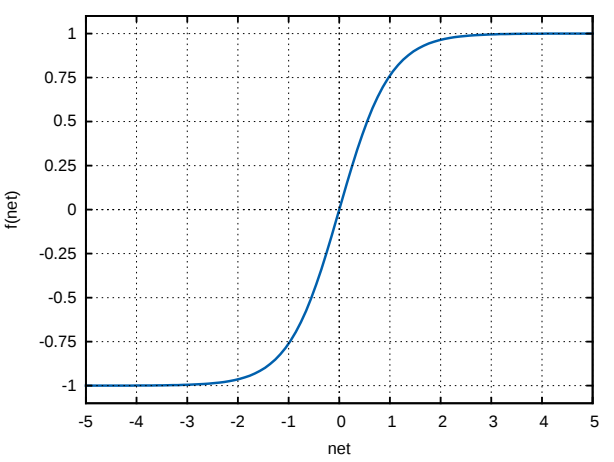
\includegraphics[scale=0.22]{img/tanh-fun.png}
                \end{subfigure}
                \begin{subfigure}
                    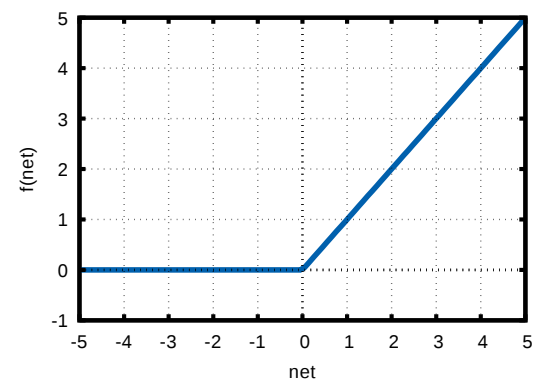
\includegraphics[scale=0.255]{img/relu-fun.png}
                \end{subfigure}
                \begin{subfigure}
                    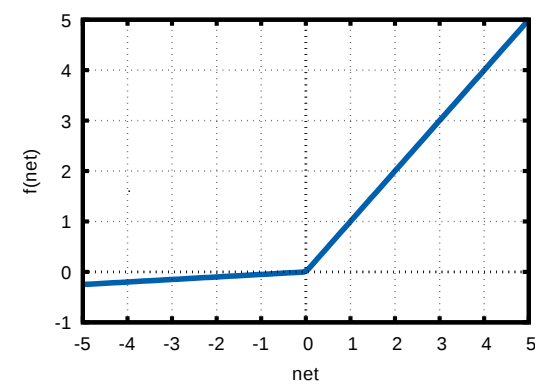
\includegraphics[scale=0.255]{img/lrelu-fun.png}
                \end{subfigure}
            \end{figure}
        \end{frame}
    
    \subsection{Unaprijedna neuronska mreža}
        \begin{frame}{Unaprijedna neuronska mreža}
            \begin{itemize}
                \item Unaprijedna višeslojna potpuno povezana umjetna neuronska mreža (engl. \textit{feedforward multilayered fully connected artificial neural network})
                \item Operacija \textbf{mapiranja} ulaza na određene izlaze
                \item Često se referira kao \textbf{višeslojni perceptron}
                \item Naziv \textbf{perceptron} prvi je upotrijebio 1958.\ znanstvenik Frank Rosenblatt u svojem radu \textit{The perceptron: a probabilistic model for information storage and organization in the brain}
                \item Ponukan MCP neuronom i Hebbovim principom učenja razvija prvi algoritam učenja \textbf{jednoslojnog perceptrona} koji nije upotrebljiv nad višeslojnim perceptronima zbog čega je dosta kritiziran
                \item Može sadržavati proizvoljnu arhitekturu, npr.\ 2x3x2:
            \end{itemize}
        \end{frame}
        \begin{frame}{Unaprijedna neuronska mreža}
            \begin{itemize}
                \begin{figure}
                    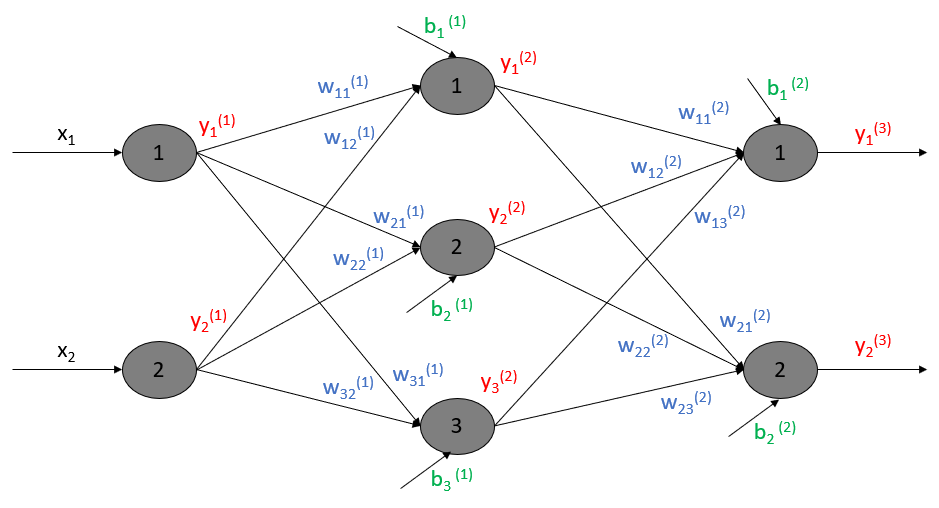
\includegraphics[scale=0.35]{img/ffann.png}
                \end{figure}
                \item \textcolor{myblue}{w\textsubscript{jk}\textsuperscript{(l)}} : težina između k-tog neurona (l--1)-vog sloja i j-tog neurona l-tog sloja.
                \item \textcolor{mygreen}{b\textsubscript{j}\textsuperscript{(l)}} : bias j-tog neurona l-tog sloja.
                \item \textcolor{red}{y\textsubscript{j}\textsuperscript{(l)}} : izlaz j-tog neurona l-tog sloja.
            \end{itemize}
        \end{frame}
        \begin{frame}{Unaprijedna neuronska mreža}
             \begin{itemize}
                \item Provedba algoritma unaprijedne neuronske mreže je računalno dosta prihvatljivo jer se cijeli postupak može prikazati matričnim računom: \smallskip
                \[\Vec{y}\textsuperscript{ (l+1)} = g(\Vec{net}\textsuperscript{(l+1)}) = g(\textbf{W}\textsuperscript{(l)} \cdot \Vec{y}\textsuperscript{ (l)} + \Vec{b}\textsuperscript{ (l)})\]
                \item \textbf{W}\textsuperscript{(l)} : matrica svih težina l-tog sloja gdje su retci težine iz svih neurona (l--1)-vog sloja u jedan neuron l-tog sloja.
                \item $\Vec{b}\textsuperscript{ (l)}$ : vektor svih bias vrijednosti l-tog sloja.
                \item $\Vec{net}\textsuperscript{(l)}$ : vektor svih net vrijednosti l-tog sloja.
                \item $\Vec{y}\textsuperscript{ (l)}$ : vektor svih izlaza l-tog sloja.
                \smallskip
                \item Važno je napomenuti da neuronska mreže mora raditi s normaliziranim podatcima jer inače neće davati dobre rezultate
             \end{itemize}
        \end{frame}
    
    \subsection{Učenje unaprijedne neuronske mreže}
        \begin{frame}{Učenje unaprijedne neuronske mreže}
            \begin{itemize}
                \item Učenje algoritmom \textbf{gradijentni spust} (engl. \textit{gradient descent}):
                \[x \leftarrow x - \alpha \cdot{\frac{\partial}{\partial x}}f(x)\]
                \item Učenje algoritmom \textbf{propagacije pogreške unatrag} (engl. \textit{Backpropagation algorithm}) : računanje parcijalnih derivacija za algoritam gradijentni spust
                \item 1986.\ Rumelhart zajedno s dvojicom prijatelja u svojem radu \textit{Parallel Distributed Processing} po prvi put definira termin \textit{Backpropagation} i učenje višeslojnog perceptrona
                \item Za učenje je potrebno definirati funkciju kazne koju je potrebno minimizirati, odnosno pronaći one vrijednosti težina za koje je iznos funkcije kazne minimalna
                \item Razmatramo funkciju kazne koja je jednaka polovici srednjeg kvadratnog odstupanja između svakog željenog izlaza mreže i stvarne vrijednosti koju mreža generira na izlazu i to kumulativno za sve raspoložive uzorke:
            \end{itemize}
        \end{frame}
        \begin{frame}{Učenje unaprijedne neuronske mreže}
            \[E = \frac{1}{2N}\sum\limits_{s=1}^N\sum\limits_{i=1}^m(d\textsubscript{s,i} - y\textsubscript{s,i}\textsuperscript{(L)})^2\]
            \begin{itemize}
                \item \textit{N} predstavlja broj uzoraka, \textit{m} predstavlja broj izlaznih neurona, \textit{d}\textsubscript{s,i} predstavlja željeni izlaz i-tog neurona s-tog uzorka, a \textit{y}\textsubscript{s,i}\textsuperscript{(L)} predstavlja stvarni izlaz i-tog neurona s-tog uzorka
                \item Potrebno je ažurirati težine sljedećim pravilom:
                \[w\textsubscript{jk}\textsuperscript{(l)} \leftarrow  w\textsubscript{jk}\textsuperscript{(l)} - \alpha \cdot{\frac{\partial E}{\partial w\textsubscript{jk}\textsuperscript{(l)}}}\]
                \item Na prvu izgleda kao da je to moguće izvesti klasičnim računom traženja parcijalnih derivacija, no mreže su često jako kompleksnih arhitektura i takav postupak bi resursno i vremenski bio prezahtjevan, stoga tu nastupa algoritam propagacije pogreške unatrag
            \end{itemize}
        \end{frame}
        \begin{frame}{Učenje unaprijedne neuronske mreže}
            \begin{itemize}
                \begin{enumerate}
                    \item[\textbf{1.}] Ciklički prolazi kroz svih \textit{N} uzoraka za učenje, jedan po jedan.
                    \item[\textbf{2.}] Ponavljaj dok nije zadovoljen uvjet zaustavljanja.
                    \item[\textbf{3.}] Za svaki uzorak iz skupa uzoraka za učenje čini:
                    \begin{enumerate}
                        \item[\textbf{1.}] Postavi uzorak na ulaz neuronske mreže i izračunaj izlaze za sve neurone primjenom formule unaprijedne neuronske mreže.
                        \item[\textbf{2.}] Izračunaj pogrešku svakog od neurona izlaznog sloja po formuli: \[\delta\textsubscript{s,j}\textsuperscript{(L)} = g'(net\textsubscript{s,j}\textsuperscript{(L)})\cdot(d\textsubscript{s,j} - y\textsubscript{s,j}\textsuperscript{(L)}).\]
                        \item[\textbf{3.}] Vraćaj se sloj po sloj i izračunaj pogreške svakog neurona po formuli:
                        \[\delta\textsubscript{s,j}\textsuperscript{(l)} = g'(net\textsubscript{s,j}\textsuperscript{(l)})\cdot\sum\limits_{i=1}^m\delta\textsubscript{s,i}\textsuperscript{(l+1)}\cdot w\textsubscript{i,j}\textsuperscript{(l)}.\]
                        \item[\textbf{4.}] Ažuriraj težine po formuli:
                        \[w\textsubscript{jk}\textsuperscript{(l)} \leftarrow w\textsubscript{jk}\textsuperscript{(l)} + \eta\cdot\sum\limits_{s=1}^N \delta\textsubscript{s,j}\textsuperscript{(l+1)} \cdot y\textsubscript{s,k}\textsuperscript{(l)}.\]
                        \item[\textbf{5.}] Ažuriraj biase po formuli:
                        \[b\textsubscript{j}\textsuperscript{(l)} \leftarrow b\textsubscript{j}\textsuperscript{(l)} + \eta\cdot\sum\limits_{s=1}^N \delta\textsubscript{s,j}\textsuperscript{(l+1)}.\]
                    \end{enumerate}
                \end{enumerate}
            \end{itemize}
        \end{frame}

\section{Rezultati}	
	\begin{frame}{Rezultati}
		\begin{itemize}
		    \item U sklopu rada implementirano je grafičko korisničko sučelje kroz koje se interaktivno unose točke u 2D koordinatnom sustavu te se iste predaju neuronskoj mreži na učenje
		    \item Točke su normalizirane tako da su se stvarne koordinate podijelile sa stvarnom širinom, odnosno visinom prozora kako bi se dobili brojevi iz intervala $[0,1]$
		    \item Težine i biasi su inicijalizirane pomoću Xavier inicijalizacije i to tipom normalne razdiobe gdje očekivanje iznosi 0, a standardna devijacija iznosi $\sqrt{\frac{1}{n\textsuperscript{(l-1)}}}$. Nazivnik predstavlja broj neurona u prijašnjem sloju.
		    \item Moguće je izabrati 3 različita razreda pri unosu točaka gdje svaki razred predstavlja svoju boju iz RGB raspona
		    \item Interno je svaki razred kodiran sa svojim kodom pa tako točka pripada crvenom razredu ako mreža na izlazu generira $[1, 0, 0]$, zelenom razredu ako generira $[0, 1, 0]$ i plavom razredu ako generira $[0, 0, 1]$
		\end{itemize}
	\end{frame}
    \begin{frame}{Rezultati}
        \begin{itemize}
            \item Mreža naravno neće davati tako okrugle brojeve pa ih je potrebno zaokružiti sljedećim pravilom: ako je izlaz manji ili jednak 0.5, onda ga postavi na 0, inače na 1. Tako će npr.\ izlaz $[0.6, 0.3, 0.1]$ biti transformiran u $[1, 0, 0]$ te će se uzorak klasificirati kao da pripada crvenom razredu
            \item Boja svakog uzorka grafičkog sučelja se određuje tako da se uzmu onoliki postoci svake od komponenata RGB koji se generiraju na izlazima. Tako će npr.\ izlaz $[0.6, 0.3, 0.1]$ poprimiti 0.6 crvene boje, 0.3 zelene boje i 0.1 plave boje.
            \item Prije učenja je moguće izabrati tri različite aktivacijske funkcije koje djeluju samo na skrivenim slojevima, dok se na izlaznom sloju nalazi funkcija \textbf{\textit{softmax}} koja na temelju svih izlaza generira postotke pripadnosti svakom od razreda gdje vrijedi da je suma svih postotaka potpuna i iznosi 100\%
            \item U nastavku su dani primjeri linearne i nelinearne klasifikacije kao i primjer prenaučenosti
        \end{itemize}
    \end{frame}
    \begin{frame}{Rezultati}
        \begin{figure}
            \begin{subfigure}
                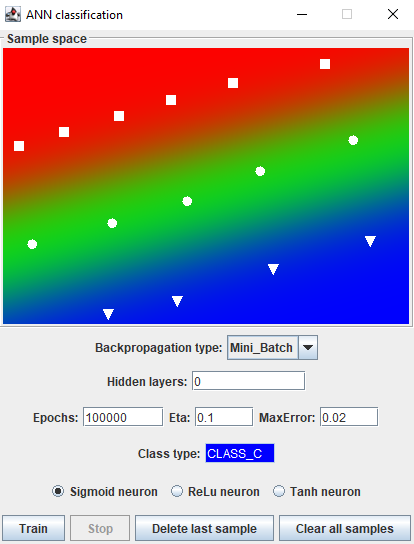
\includegraphics[scale=0.4]{img/jednoslojni_lin.png}
            \end{subfigure}
            \begin{subfigure}
                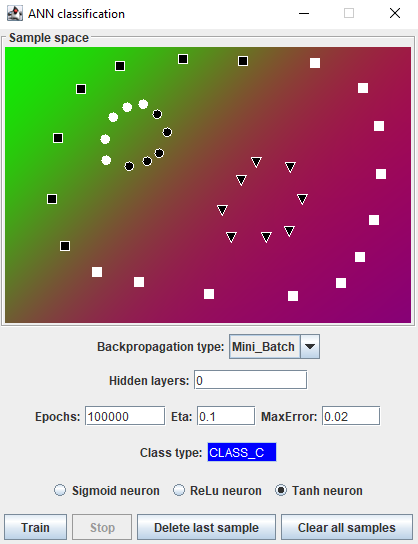
\includegraphics[scale=0.4]{img/jednoslojni_nelin.png}
            \end{subfigure}
        \end{figure}
    \end{frame}
    \begin{frame}{Rezultati}
        \begin{figure}
            \begin{subfigure}
                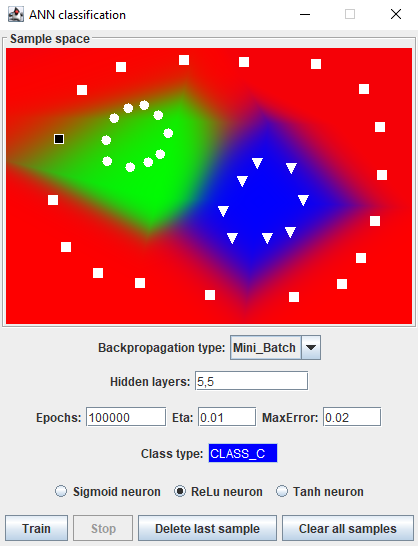
\includegraphics[scale=0.4]{img/viseslojni_nelin.png}
            \end{subfigure}
            \begin{subfigure}
                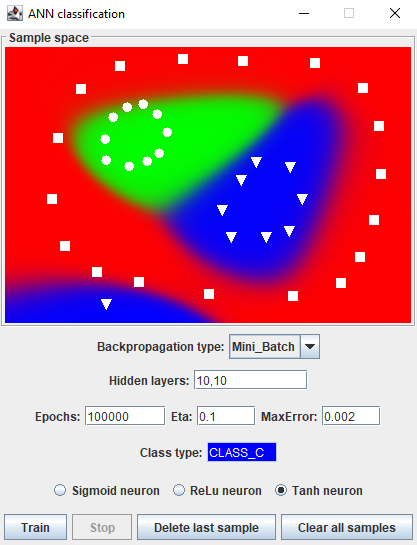
\includegraphics[scale=0.4]{img/pretreniranost.png}
            \end{subfigure}
        \end{figure}
    \end{frame}

\section{Zaključak}
	\begin{frame}{Zaključak}
		\begin{itemize}
	        \item Za rješavanje određenih problema treba jako dobro poznavati teoriju koja se krije iza algoritma umjetnih neuronskih mreža
	        \smallskip
			\item Pametna inicijalizacija težina je jako bitna za postizanje dobrih rezultata unaprijednom neuronskom mrežom kao i odabir arhitekture te aktivacijskih funkcija 
		\end{itemize}
		
		\bigskip		
		\pause		
		
		\begin{block}{Mogući nastavci na ovaj rad}
			\begin{itemize}
				\item Proučiti inačice algoritma propagacije pogreške unatrag te ih znati primijeniti na probleme koje rješavamo
				\item Upoznati se s dubokim neuronskim mrežama i algoritmima dubokog učenja
			\end{itemize}
		\end{block}
	\end{frame}

\end{document}